%!TeX spellcheck = en-US

\chapter{Web Genre Identification: A Survey}

\label{chap:relevant_work}

%----------------------------------------------------------------------------------------

% Define some commands to keep the formatting separated from the content
\newcommand{\keyword}[1]{\textbf{#1}}
\newcommand{\tabhead}[1]{\textbf{#1}}
\newcommand{\code}[1]{\texttt{#1}}
\newcommand{\file}[1]{\texttt{\bfseries#1}}
\newcommand{\option}[1]{\texttt{\itshape#1}}

%----------------------------------------------------------------------------------------

\section{Introduction}\label{chap:relevant_work:sec:intro}

The notion of \textit{Genre} in linguistics domain is an abstract taxonomy of the \textit{texts}, on which there is a great theoretical and mostly philosophical debate respectively to its internal mechanics of this taxonomy evolution. In computational linguistics domains is yet an other taxonomy where several computational methodologies has been developed for automating the process. All these methods are mainly based on \textit{Machine Learning (ML)} where most of the work historically has been focused on the raw text pre-processing and the feature selection methodologies. In addition, mostly out-of-the-box ML methods has been tested and some of its variations. Only recently there is a redirection of the research focus to the \textit{Vocabulary Learning Models (VLM)} which are used for feeding the input of the Identification or Classification ML models, instead of the \textit{Bag-of-Words (or Bag-of-Terms) BoT }\footnote{In this text Bag-of-Terms (BoT) is equivalent to the Bag-of-Words  (BOW), which has been widely used in the literature of the Information Retrieval and Natural Language Processing domains. Since, BoT is accurately describing the meaning of BOW in most of the cited literature.} model. This study is focude mostly on the Web-Genre Identification (WGI) computational methodologies, which is the main focus of the Natural Language processing and Information Retrieval research focus, in respect of the genre notion. Although there a several other text resources, other than the Web, where the Automated Genre Identification (AGI) has been also been studied and also are cited here.

Genre means "genus" in the Greek language and for the text focused studies (either traditional linguistics or computational) means style. The main utility of the genre taxonomy, or in other words the reason we like as humans to categorize and give a "genus" to our text is for speeding up the communication. Thus, what we mostly do with texts is to use a genre taxonomy for transferring or retrieving the information in the "speed" of a word (or word n-gram) when it comes to describe the texts.....

\textbf{NOTE: In this survey section the Genre and Web-Genre is studied mostly thematically than historically. However, wherever there is interesting historical sequence in the research field it is pointed out.}


Since 2013 the where two very informative research studies related to the utility, evolution, and recognition of the genre taxonomy. One (REF) from the discipline of the \textit{English for Academic Purposes} (EAP) where it was vividly discussed the divergence in the genre taxonomies between the difference academic disciplines and reasoned the utility of the genre taxonomy for enabling the teachers and the students to improve their rhetorical and written language with the purpose of improving the teaching procedure. What is important to note for this study is the conclusion that the same genre-type can be very different for the communication purpose, i.e. as text identity carrier, but it can also contain the same style and other language properties when the purpose is similar, for example the article of new paper and an article form a magazine where one can claim that they are a different genre-type although they governed by the same linguistic properties.

*** Genre variations in student .... (paper)
The types of their study genre taxonomy mainly focused on the \textit{purpose} of the students written context and less on the \textit{style}, thus their genre-types where \textit{Creative Writing, Response Paper, Critique/Evaluation, Argumentative Essay, Report, Research Paper and Proposal}. Their study was a manual statistical process, similar to a \textit{Data Mining} process where grammatical features were counted in the texts. Then these features where indicating the score for each of the four (4) dimensions which has been qualitatively predefined. The counting process was using a heuristic computational tagger, named as Biber tagger (see Biber 1988 or ???).   

On the other hand and other research lying in the discipline of cognitive computing an health research they found humans are recognizing the genre type of a document or web-page using other cognitive processes relates mostly to the formatting of the text. Particularly they used as well configured apparatus for tracking the eyes movement while the recognition effort, where they fount that the eyes where following specific paths and where stopping to special landmarks on the text. They have concluded that the process of genre recognition was mostly related to the format and not the context, in addition they statistically measured that they previews experience was not related to the recognition process. Although it was the previews knowledge of the text formatting was accelerating the process. However, on the opinion of the authors of this study the genre recognition is a more deep process, thus as one can concluded by reading their study the landmarks they are referring into seems to be the only context combined with the formatting of the text that the human brain is requiring for identifying the genre-type. Given that their study is focused on the e-mail genres where formatting options compare to the web or textbooks is rather limited is advocating the conclusion that the minimum context is required for identifying the genre-type.

They are discussing of tree main perception (psychology) theories, i.e. Gestaltism (or Gestalt psychology), Ecological and Constructivism, which are the theories which can interpret the perception procedures, it this case the eye movement on the texts, to the cognition process for identifying the genre types of the texts. The perception procedure includes some eye movements mainly doing two tasks, \textit{scanning} and \textit{skimming}. Theses two procedures are irrespective of the belief of the supported interpretation theory related to the internal thought process for making a genre taxonomy decision. Scanning is the process where more or less we are trying to locate information of interest where the information has a homogeneous property, such as the a phone number in phone-book list. Skimming is the process where we are trying to locate information of interest where the information is raw or without a specific form, such as names, verbs, or phrases that is related to the abstract related concept in order to decide whether the text is matches and worth farther reading. 

The process of scanning and especially skimming in practice follows some specific eye movements, i.e. Fixation and Saccadic. Saccadic is the process while scanning or skimming that the eye is jumping around to the text, while Fixation is the process where the eye remains focused for a while. One can resemble the process like navigation where the eye is constantly moving while is focused for small fragments of time in landmarks of interest.

\begin{figure}[t]
	\begin{center}
    	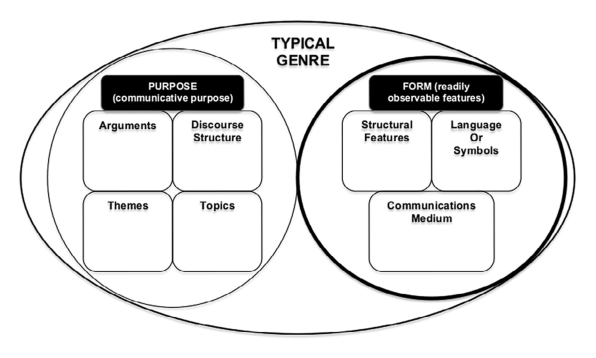
\includegraphics[scale=0.95]{Figures/Sotlen_diagram.eps}
		\caption{Stolen Imag.}
		\label{fiig:Stolen}
	\end{center}
\end{figure}

***
Genres, in textual sense, is sometimes defined as group of texts of documents that share a communicative purpose, as determined by the \textit{discourse community} which produces and/or reads them. "In \textbf{structurational}terms, genre are social institutions that are produced, reproduced, reproduced or modified when \textit{human agents} draw on genre rules to engage in organizational communication".

"Layout in organizational communities cause people to focus perceptually on key parts of the text and our \textbf{empirical research has previously demonstrated that people use layouts and other related cues to focus on key parts of the text.}"
***

A very recent research on Cross-Lingual Genre Classification showed that it is possible to get very good results when an ML model is trained with a corpus samples of one language and then testing the trained model to an other. However, the evaluation framework was closed-set and the relation of the languages seems to be of a great importance for the accuracy performance of the model. That is, in some cases it was important the language to be of the same group for example the Roman or the Slavic group of languages and for others was not. Some times oddly the performance was dropping when the language was form the same language group \parencite{nguyen2019cross}.

Web Genre Identification (WGI) concerns the association of web pages with labels that correspond to their form, communicative purpose and style rather than their content. The ability to automatically recognize the genre of web documents can enhance modern information retrieval systems by enabling genre-based grouping/filtering of search results or building intuitive hierarchies of web page collections combining topic and genre information \parencite{Braslavski2007,Rosso2008,de2009genre}. For example, a search engine can provide its users with the option to define complex queries (e.g., blogs about machine learning or eshops about sports equipment) as well as the option to navigate through results based on genre labels (e.g. social media pages, web shops, discussion forum, blogs, etc). The recognition of web genre can also enhance the effectiveness of processing the content of web pages in information extraction applications. For example, given that a set of web pages has to be part-of-speech tagged, appropriate models can be applied to each web page according to their genre \parencite{Nooralahzadeh2014}. However, research in WGI is relatively limited due to fundamental difficulties emanating from the genre notion itself.

\textbf{The most significant difficulties in the WGI domain are: (1) There is not a consensus on the exact definition of genre \parencite{crowston2011problems}; (2) There is not a common genre  palette that comprises all available genres and sub-genres \parencite{santini2011cross,mehler2010genres_on_web,mason2009n,sharoff2010web}, moreover, genres are evolving in time since new  genres are born or existing genres are modified \parencite{Boese2005}; (3) It is not clear whether a whole web page should belong to a genre or sections of the same web page can belong to  different genres \parencite{jebari2015combination,madjarov2015web}; (4) Style of documents is affected by both genre-related choices and author-related choices \parencite{petrenz2011stable,Sharroff2010}. As a result, it is hard to accurately distinguish between personal style characteristics and genre properties when style is quantified.}

As \textit{Web Search} from an extension of IR because the main subject under investigation \parencite{manning2008introduction}, \textit{Web page Genre Classification } is becoming the main subject of document classification research.

Most previous work in WGI follows a typical closed-set text categorization approach where, first, features are extracted from documents and, then, a classifier is built to distinguish between classes. Attention is paid to the appropriate definition of features that are able to capture genre characteristics and should not be affected by topic shifts or personal style choices. 

Blogs is a genre-type has attracted as special interest on its own, in differed domains such as in sociology, psychology, linguistics and mostly in computational linguistics and WGI. There are several blogs' properties of interest of the research and  also blogs having their own sub-genre taxonomy. Blog-taxonomy general genres are \textit{Filter, Personal-diary} and \textit{Notebook} and other related to the authors group of styles such as \textit{Reflective, Narrative, Emotional, Rational} and \textit{Personal , Non-Personal}. The thought research on the blog-types classification has delivered a set of special linguistic and web-page structural properties which are increasing the performance of the closed set classification. Details for this linguistic properties used for specially for blogs sub-taxonomy classification are described in section \ref{chap:relevant_work:sec:features:subsec:heuristics} \cite{virik2017blog,hoffmann2012cohesive,hoffmann2012cohesive,derczynski2014social,qu2006automated}. 

\section{Genre Definitions: The Linguistics and the Computational Linguistics}\label{chap:relevant_work:sec:linguistics_definition}

Overcoming the difficulties related to the genre taxonomy pointed out in linguistic and empirical studies, in text in \textit{text categorization} there is a great amount of work related to the automated categorization of texts based on \textit{genre taxonomy}. Although, starting from fundamentally different routes computational and linguistic studies, both ended up with the same notion of genre, which is eventually having two complimentary meanings,  i.e. \textit{Style} and \textit{Genus}\footnote{Genus in Greek means \textit{type} or \textit{class}} \parencite{sugiyanto2014term}. 

(DEFINITION DEBATE) In linguistic studies there is a great debate in defining \textit{the notion of genre} as an \textit{abstract categorization} of texts and the relation between them. Despite the methodological differences the linguistic community concluded that the idiosyncrasy of the \textit{genre taxonomy} is mutable and diverse \parencite{coutinho2009describe}. This kind of idiosyncrasy is yielded to the \textit{genre taxonomy} due to the spontaneous genesis of the genre classes. The genesis of a genre class is socio-centric interaction which is emerging from the need to describe the texts in order to accelerate the social communication procedure. Thus, genre classes are spontaneously emerging while the communication procedure is taking place.

(READERS PERCEPTION) Humans can efficiently recognize the genre-types by processing the texts intuitively. However, there is a \textit{great luck of consensus} for the genre-types, particularly naming the genres. There there was an effort of several user studies for eliciting the mechanics in the process of \textit{genre identification and tagging}. The results on user agreement were very discouraging. Also, when it come to the reporting, i.e. for humans to describe specifically the terms or/and the attributes with which they use to identify the genre-types then there is a great confusion. A convincing reasoning for that is the plethora of textual, stylistic and conceptual terms which are used where they are different per individual and/or per group (e.g. teachers, scientists, engineers) for the same (or similar) text (or web-page) \parencite{roussinov2001genre, crowston2011problems}. 

Researchers, of cognitive computing and health research disciplines, found humans are recognizing the genre type of a document (or web-page) using other cognitive processes related mostly to the form of the text. Particularly they used as well configured apparatus for tracking the eyes movement while the recognition effort. One can resemble the process like navigation where the eyes are constantly moving while they are focusing for small fragments of time in landmarks of interest. The pausing of the eyes on the text "landmarks" is called \textit{Fixation} while the "jumping" movements of the eyes is called \textit{Saccadic}. The whole process was the effort to locate information of interest such as a specific text forms, names, verbs, or phrases that are related to the abstract concept in order to decide whether the text is matches and worth farther reading. They systematically found that the process of finding the genre-type of the text is the same as to find out whether a text worth farther reading. Thus, the genre taxonomy definitely accelerates the communication procedure and helping the reader of the text find the information of interest faster \parencite{clark2014you}.

(WRITERS AWARENESS) In discipline of the \textit{English for Academic Purposes} (EAP)  it was vividly discussed the divergence in the genre taxonomies between the difference academic disciplines and reasoned the utility of the genre taxonomy for enabling the teachers and the students to improve their rhetorical and written language with the purpose of improving the teaching procedure. What is important to note for this study is the conclusion that the same genre-type can be vary differently form the communication purpose, i.e. as text identity carrier, but it can also contain the same style and other language properties when the purpose is similar, for example the article of new paper and an article form a magazine where one can claim that they are a different genre-type although they governed by the same linguistic properties. Therefore, for the witter of a text is is very important to be aware (thus to be taught) of the genre-type in order the text to be recognizable for the reader is seeking similar texts \parencite{hardy2016genre,melissourgou2017genre,al2017genre}.

(NEWS GENRE SUB-GENRES) The utility of the text genre identification (and/or classification) has been realized by the journalism historians. The technology advances and the new science innovations cased the attraction to the field. Journalism historians using a different genre-taxonomy where they mainly focusing on the purpose of the texts by analyzing the structure of the texts, where the structure consist of abstract elements. Their main genre-type are Inverted Pyramid, Martini Glass, Kabob, Narrative, Narrative and elements are \textit{Standard Lede, Body Section,  Narration, Synopsis, Image Lede}.  Similarly to the EAP domain, their sub-genre taxonomy is including genre-types like . \parencite{dai2018fine}.

(GENRE AS WRITING STYLE) The aforementioned variations of the genre taxonomy's notion is related more to the methodology and the objective of the text categorization task's specifications, rather than the philosophical difference. Particularly in author attribution domain there is a focus on identifying the \textit{style of the author} \parencite{stamatatos2009survey,koppel2011authorship,koppel2014determining}. On the other hand in the information retrieval (IR) domain, the interest is to classify the texts based on a predefined \textit{genre pallet}. Thus the interest is focused on the \textit{style of the authors group}, such as scientists, journalists, bloggers, etc.

(THE WEB GENRE) In consideration of \textit{the web genres taxonomy} it has been also eloquently analyzed the utilities and the difficulties for the web users. It has been pointed out that the genre taxonomy is summarizing the type and the style of the text in a single term as a communicative act [This conclusion cited also in \parencite{de2009genre}]. In the domain of \textit{web genre identification (WGI)}, \textit{the web genre taxonomy pallet} (which mostly used for research) has been formed in a top-down approach, where a group of experts are forming the taxonomy based on the specific objective of the task \parencite{crowston2011problems}. Moreover, in WGI research there was a very early observation that genre are organized in a hierarchical manner \parencite{wu2010fine}. Thus, most likely a web page might be multi-genre, the genre unit is considered to be the web-page \parencite{madjarov2015web,jebari2015combination}. However, in section \ref{???} there is a discussion related the web-genre units other than the web-page.

As described so far, after a significant amount of work related to the study of the \textit{Genre-Taxonomy} and the \textit{Genre-Identification}, there is an agreement for the criteria which are defining the genres and the  web-genres. That is, the \textit{Form} and the \textit{Function/Purpose}. Complimentary criterion is the \textit{Context}, for example, the genre-type of the \textit{academic home web-pages} are easily identified by their context. The computational process of a text's \textit{context} is a standard procedure for the \textit{Topic Identification}. Although text's topic is considered as orthogonal to its genre, in cases such as academic home web-pages some context indicators can be exploited for the identification, also, of the Genre \parencite{coutinho2009describe,crowston2011problems,kanaris2009learning,jebari2015combination,gollapalli2011identifying}. 

Considering the above, it is clear that the Web-Genre Taxonomy has also a relatively abstract notion where is slightly changes depending on the research framework, despite the fact that the criteria for the genre-types of the texts are more or less common. Thus, for continuing the a this study in for the computationally, particularly NLP, research approach we are defining the notion of web-genre-type as follows.   

\textbf{However, \textit{genre} itself requires different level of human reading abilities to be recognized and even with these skills different humans may disagree \parencite{mccarthy2009psychological}.}

\begin{definition} Web-Genre-Type is defined as a class where its samples are i.i.d. Thus every web-unit (usually web-page) is always derived under a unique class distribution and the class distributions are not overlapped. That is, the Genre-Taxonomy consist from a distinctive non-overlapping classes/types.
\end{definition}

\section{Machine-Learning Methodology for Web Genre Identification and Classification}\label{chap:relevant_work:sec:machine_learning_methods}

\textbf{(SVM Based)} There are several studies where their perdition model was the infamous SVMin the closed set framework, either in multi-class or binary form \parencite{dai2018fine}. 

SVM, Naive Bayes, Random Forest, Decision Trees(C4.5), AdaBoost and several types of features.\parencite{lee2017text}. Where Random Forest and SVM were the top performing classification methods for the genre-classification task.

SVM closed-set classification was also used for cross-lingual closed-set classification \parencite{nguyen2019cross}. 

In \parencite{virik2017blog} SVM is compared with Naive Bayes Classifier and k-Nearest Neighbours on the classification accuracy for the Blogs' sub-genre taxonomy. Their preliminary analysis on the correlation of the linguistic features and the sub-genres of the blogs indicating that all three algorithms were expected to be successfully, however, SVM was a bit better in performance. 

It seems than SVM based algorithms are high performance learners for the genre and web-genre closed-set classification task either in the multi-class or in the binary form. However, in the case of the open-set classification the performance drops significantly as shown in several studies such as ..., where simpler ensembles based models seems to work with higher performance. 

Finally, we design news structure indicative features and train a Support Vector Machine (SVM) (Cortes and Vapnik, 1995) classifier to label each news article with one of the proposed news structures. Experimental results show that reasonable performance can be achieved for automatic structure-based news genre classification by using our structure indicative features, even though results on minority classes remain low.

Although, the traditional bag-of-words approach had better result with XABoost or other techniques been tested for over a decade on genre identification or/and particularly on WGI, distributional feature models are early showing their advantages over the TF-IDF (or TF alone) models[REF].

Additionally, other methods extending the ensembles methodology like Random Forests have been alo became popular[REF].

Concerning the classification models involved in WGI studies, when a given genre taxonomy is utilized and there is no noise, then well-known machine learning models, like SVMs, decision trees, neural networks, naive Bayes, Random Forests, etc. are used \parencite{Lim2005,santini2007automatic,kanaris2009learning,jebari2015combination,sharoff2010web}. In case of presence of  noise, in a clustering framework described in \parencite{kennedy2005automatic} one cluster is built for each predefined class and another cluster is built for the noise. However, the most  common approach to handle noise is to build binary classifiers where the positive class is based on a certain predefined category and the negative class is based on the concatenation of  all other predefined categories plus the noise \parencite{kennedy2005automatic,dong2006binary,levering2008using}. Such a combination of binary classifiers can also be seen as a multi-label  and open-set classification model where a web page can belong to different genres and it is possible for one page not to belong to any of the predefined genres. More concrete open-set  classification models for WGI were presented in \parencite{stubbe2007genre,pritsos2013open}. However, these models were only tested in noise-free corpora \parencite{pritsos2015clef}. More  recently, Asheghi \parencite{Asheghi2015} showed that it is much more challenging to perform WGI in the noisy web in comparison to noise-free corpora.

To begin with, Kanaris and Stamatatos \parencite{kanaris2009learning} recently proposed a method for extracting an \textit{variable length n-gram corpus dictionary} for training an SVM model with a sample points projected in a feature space defined by this dictionary. The dictionary composed from a mixture of 3-grams, 4-grams and 5-grams, carefully selected from a modified version of \textit{LocalMaxs }algorithm. The algorithm was using a \textit{``glue function''} for selecting the most informative n-grams and the rest of them where discarded. Their \textit{``glue''} function was based on the frequency of n-grams in the corpus and not to any other feature selection method such as \textit{information gain}, in order to be portable to other corpora for farther evaluation.  

\textbf{(Distance Based)}

\textbf{(Neural Based)}
Recently Neural Networks have been used for modeling the WGI task (and other text classification tasks), additionally or independently of the Vocabulary modeling where neural-models have widely used. 

Most notably is the used of Recurrent Neural Networks (RNN) where Linguistic Complexity Contours (LCC) where employed as modeling features (LCC details are explained in section \ref{chap:relevant_work:sec:intro:subsec:heuristics}). Their model was based on 32 LLC features where fed to 32 Gated Recurrent Units (GRU)  and the output of each GRU was also fed to the next. Then all the output GRU output was the input of a Dense Layer of the RNN where a Softmax decision function was applied on. Their model was a closed-set framework with very high performance where was reaching over $90\%$  accuracy. (\parencite{strobel2018text}

\textbf{(Ensemble Based)} 
There are very few \textit{ensemble based} algorithms employed for the WGI and AGI task, however, they seem to be a very promising path as shown in \cite{onan2018ensemble,pritsos2015clef,pritsos2013open,pritsos2018open}. Particularly there are three methods, mainly, where an ensemble can be formed, namely, AdaBoost, Bagging and Random Feature (RFS) Subspace ( (i.e. random sub-sampling). In this study we mainly focusing on the RFS, it is one of the algorithms are thoroughly presented in the context of WGI/AGI task.

\textit{AdaBoost} is a \textit{Boosting} algorithm where usually a random sampling is performed over the data and s set of classifier are trained over these samples. There is a weighting scheme over the samples which is changing in every training iteration, where for the samples mostly miss-classified, by most of the learners, their weights are increasing. In this manner the difficult samples repetitively to classification are presented to the weak learner in more iterations in order the whole systems of learners fit adjust better over these samples.

\textit{Bagging/Bootstrap aggregating} is an ensemble learning methods where a set of independent learners are training on different subsets of samples. Sampling with replacement is employed for Bagging, usually random. The performance of the ensemble is significantly influenced by the sampling policy/model. The ensembles decision is obtained either by the majority voting or my the weighted voting for a random sample.

\textit{RFS } is mainly similar to Bagging in respect the sampling policy might be used. However, they deffer in the decision method where in RFS there is a \textit{$\kappa$ metric} or a \textit{$\sigma$ threshold} for the agreement of the weak learners for a random sample. This method also can be used for closed-set and open-set multi-class classification methods such as RFSE algorithms will be discussed in section \ref{}.

In \parencite{chen2012genre} an open-set ensemble presented where two multi-class SVM classifiers where trained for all the genres of their special formed genre-taxonomy for \textit{office documents} (details for office documents taxonomy find in \ref{}). Every SVM classifier was trained in a different mutually exclusive training subset, where the other part of the training set was used for tuning and vice-versa. The assumption of this training methods is that part of the support vectors  will be optimized for every SVM preserving the generalization of the two independent models and the combined classification will manage to fit well over the whole corpus. Their ensemble's decision rule as shown in equation \ref{eq:office_doc_ensemble} is a pairwise genre-class operation for an arbitrary page, where the truth table of this binary rule for all genre-class pairs might end up wilt all $0$ (zero) outcome. Then this page remains as unknown in all other cases at least one genre will return as true. On this combination rule several application can be operated as they have presented.


\begin{equation}\label{eq:office_doc_ensemble}
	(g^{k}_{1}[i] \vee g^{k}_{2}[i])  \wedge  (g^{m}_{1}[i] \vee g^{m}_{2}[i]) ,   \forall m \neq k
\end{equation}
where $\{k, m\}$ are the genre classes and $\{g_{1}, g_{2}\}$, are the genre SVM classifiers.

The above ensemble is an \textit{Early Fusion} category of ensembles where the potential different features and document representation are all combined in a sum-up vector for each document, i.e. a weighted sum or a concatenation of the different feature vectors. Then the summed-up vectors are the input for the learners of the ensemble where Bagging, Boosting, Majority voting or other strategies are used for then training and testing (or production) phases.

In \parencite{finn2006learning} a \textit{Late Fusion} ensemble is proposed for the AGI task which is an other category of ensembles. Late Fusion ensembles are composed from learners of the same model (say SVM, C4.5, NN etc) where every one is trained only on a specific feature set (or/and document representation). In the testing phase the ensemble me majority voting us a common strategy. 

Particularly the in their study they are testing C4.5 decision trees for BOW, POS, and \textit{Text Statistics} in detail explained in  section \ref{} they shown that their \textit{Multi View Ensemble }, i.e. the Late Fusion Ensemble, performs significantly better because every one of these features was a better choice only for a part of the genres in their taxonomy, thus the fusion of the all three increased the performance for all genre in total. In is important to note that in the training phase \textit{Active Learning}, and binary vector representation also were used. 

Active Learning in their study was defined as a sample selection strategy while training where an an evaluating process was indicating which sample was better to be used for the specific C4.5 learner, for the specific features set. The Late Fusion ensemble with the active learning strategy shown to be a promising proposal for the Domain Transfer problem for AGI.

\textbf{Domain transfer} is the ability to transfer across multiple-topic domains the same learner when it has been only trained in one of these domains. As an example, for the genre \textit{News} there might be several topic domains such as Sports, Technology, Science, Health, Politics. An ML model which has been trained for News only on Sports topic and still can perform similarly good for Technology, etc, it considered to perform well in domain transfer cases. This is very important particularly for AGI where usually the positive available sample for a genre are not available in a wide variate topic-domains (see section \ref{} discussing the genre taxonomy corpus building issues).




\textbf{(Clustering Based)}
(Open Set Classification)

\section{Web Genre Noise and the Open-set approach}\label{chap:relevant_work:sec:intro}
Most previous studies in WGI consider the case where all web pages should belong to a predefined taxonomy of genres \cite{Lim2005,santini2007automatic,kanaris2009learning,jebari2014pure_URL}. Putting this setup under the vantage point of machine learning, it is the same as assuming what is known as a closed-set problem definition. However, this naïve assumption is not appropriate for most applications related to WGI as it is not possible to construct a universal genre palette a priori nor force web pages to always fall into any of the predefined genre labels. Such web pages are considered \textit{noise} and include web documents where multiple genres co-exist~\cite{santini2011cross,levering2008using}. 

Santini~\cite{santini2011cross} defines \textit{structured noise} as the collection of web pages belonging to several genres, unknown during training. Such structured noise can be used as a negative class for training a binary classifier \cite{Vidulin2007}. However, it is highly unlikely that such a collection represents the real distribution of pages of the web at large. On the other hand, \textit{unstructured noise} is a random collection of pages \cite{santini2011cross} for which no genre labels are available. The effect of noise in WGI was first studied in \cite{shepherd2004cybergenre,kennedy2005automatic,dong2006binary,levering2008using}.

Open-set classification models for WGI were first
described in~\cite{pritsos2013open,stubbe2007genre}. However, these models were only tested in noise-free corpora \cite{pritsos2015clef}. Asheghi~\cite{Asheghi2015} showed that it is much more challenging to perform WGI
in the noisy web setup in comparison to noise-free corpora. Recently, \textit{Ensemble Methods} were shown to achieve high effectiveness in open-set WGI setups~\cite{pritsos2018open}.


To handle noise in WGI there are two options. First, to adopt the closed-set classification setup having one predefined category devoted to noise. Since this category would comprise all web pages not belonging to the known genre labels, it would not be homogeneous. Moreover, this noise class would be much more greater with respect to the other genres causing class imbalance problems. The second option is to adopt the open-set classification setting where it is possible for some web pages not to be classified into any of the predefined genre categories \parencite{pritsos2013open}. This setup avoids the problem of class imbalance caused by numerous noisy pages and also avoids the problem of handling a diverse and highly heterogeneous class. On the other hand, open-set classification requires strong generalization with respect to the closed-set setup \parencite{scheirer2013toward}.

Santini \parencite{santini2011cross} defines \textit{structured noise} as the collection of web pages belonging to  several genres. Such structured noise can be used as a negative class for training a binary classifier \parencite{Vidulin2007}. However, it is highly unlikely that such a collection  represents the real distribution of pages on the web. On the other hand, \textit{unstructured noise} is a random collection of pages \parencite{santini2011cross}. The effect of noise in WGI  was first studied in \parencite{shepherd2004cybergenre,kennedy2005automatic} where predefined genres were personal, organizational, and corporate home pages while noise consisted of non-home  pages. However, the distribution of pages into these four categories was practically balanced, hence it was not realistic. Dong et al.\parencite{dong2006binary} uses noise as the majority  class in an experiment where 190 instances from personal homepage, FAQ, and e-shop categories were used in combination with 600 noise pages. Similarly, Levering et al \parencite{levering2008using} uses about 200 instances for the predefined genres of store homepages, product lists, and product descriptions in combination with about 800 other pages (noise).

The majority of previous studies in WGI disregard the presence of noise. Santini \parencite{santini2011cross} defines \textit{structured noise} as the collection of web pages belonging to several genres. Such structured noise can be used as a negative class for training a binary classifier \parencite{Vidulin2007}. However, it is highly unlikely that such a collection represents the real distribution of pages on the web. On the other hand, \textit{unstructured noise} is a random collection of pages \parencite{santini2011cross}. The effect of noise in WGI was first studied in \parencite{shepherd2004cybergenre,kennedy2005automatic} where predefined genres were personal, organizational, and corporate home pages while noise consisted of non-home pages. However, the distribution of pages into these four categories was practically balanced, hence it was not realistic. Dong et al.\parencite{dong2006binary} uses noise as the majority class in an experiment where 190 instances from personal homepage, FAQ, and e-shop categories were used in combination with 600 noise pages. Similarly, Levering et al \parencite{levering2008using} uses about 200 instances for the predefined genres of store homepages, product lists, and product descriptions in combination with about 800 other pages (noise).

Concerning the classification models involved in WGI studies, when a given genre taxonomy is utilized and there is no noise, then well-known machine learning models, like SVMs, decision trees, neural networks, naive Bayes, Random Forests, etc. are used \parencite{Lim2005,santini2007automatic,kanaris2009learning,jebari2015combination,sharoff2010web}. In case of presence of noise, in a clustering framework described in \parencite{kennedy2005automatic} one cluster is built for each predefined class and another cluster is built for the noise. However, the most common approach to handle noise is to build binary classifiers where the positive class is based on a certain predefined category and the negative class is based on the concatenation of all other predefined categories plus the noise \parencite{kennedy2005automatic,dong2006binary,levering2008using}. Such a combination of binary classifiers can also be seen as a multi-label and open-set classification model where a web page can belong to different genres and it is possible for one page not to belong to any of the predefined genres. More concrete open-set classification models for WGI were presented in \parencite{stubbe2007genre,pritsos2013open}. However, these models were only tested in noise-free corpora \parencite{pritsos2015clef}. More recently, Asheghi \parencite{Asheghi2015} showed that it is much more challenging to perform WGI in the noisy web in comparison to noise-free corpora.

One of the most recent approaches related to the open-set classification on the \textit{Text Classification} problem was suggesting the reduction of the \textit{open space risk} using an SVM based methodology. Particularly, they are comparing 8 SVM based methods (additionally with an EM Semi-supervised method) in a open-set setup compare to their SVM Center-Based Similarity Space Learning SVM methods also in a open-set setup. Their method outperformed the other methods significantly with some exceptions. 

Their main contribution is the transitions of the problem form the \textit{feature space} to the \textit{distance space}. Particularly they are using ten (10) different centroids one for each of the five (5) different distance measures proposed by (Fei and Liu 2015......) and for two (2) different document representations one for uni-grams and one for bi-grams. Their centroids are calculated using  eq \ref{eq:manning_centroids} 

\begin{equation}\label{eq:manning_centroids}
	c_{j} = \frac{\alpha}{\lvert D_{+} \rvert} \sum_{d_{i} \in D_{+}} \frac{x_{j}^{i}}{\lVert x_{j}^{i} \rVert } - \frac{\beta}{\lvert D - D_{+} \rvert} \sum_{d_{j} \in D - D_{+}} \frac{x_{i}^{j}}{\lVert x_{i}^{j} \rVert}
\end{equation}

where $D_{+}$ is the set of documents in the positive class and $\lvert . \rvert$ is the size of function. $\alpha$ and $\beta$ are parameters, which are usually set empirically.

The SVM methods under testing where 1-vs-rest multi-class SVM (Platt200...), 1-vs-set Machine SVM \cite{scheirer2013toward}, W-SVM (Scheirer2014....), $P_{1}$-SVM (Jain2014), $P_{1}$-SVM (Jain2014), Exploratory Seeded K-means (Exploratory EM) (Dalvi2013...). They have also used a kind of \textit{openness testing}, by using $25\%$ to $100\%$ of the classes and their method were mostly outperforming the other methods. The macro-F1 score range of their methods from the most open set-up to the totally closed (i.e. using the $100\%$ of the classes) was from $0.417$ to $0.873$ depending on the corpus and the special class set-up \parencite{fei2016breaking}.

\section{Features (???and Dimensions???) extraction or selection}\label{chap:relevant_work:sec:features}

 To this end, several document representation features have been proposed and are related with textual content, e.g. character n-grams, word n-grams, part-of-speech histograms etc. \parencite{kumari2014web,petrenz2011stable,mason2009n,sharoff2010web} as well as the form, structure, and visual appearance of web documents, e.g., html tags, number of images, scripts etc. \parencite{Lim2005,levering2008using}. Usually, the combination of features from different sources enhances the robustness of WGI approaches \parencite{levering2008using,kanaris2009learning}.

Great attention historically on WGI has been given to the appropriate definition of features that are capable of capturing genre characteristics --- which includes but are not limited to character n-grams or word n-grams, part-of-speech histograms, the frequency of the most discriminative words, etc.  \cite{kanaris2009learning,kumari2014web,levering2008using,Lim2005,mason2009n,onan2018ensemble,petrenz2011stable,sharoff2010web}. Additionally, some additional useful features might come from exploiting HTML structure and/or the hyperlink functionality of web pages \cite{abramson2012_URL,asheghi2014semi,jebari2014pure_URL,priyatam2013don_URL,zhu2011enhance}. Recently deep learning methods have also been tested in genre detection setups with promising results~\cite{worsham2018genre}. 

A great variety of features to quantify the stylistic choices related to genre have been proposed in previous work. These are mainly based on textual content (e.g., character and word  n-grams) \parencite{mason2009distance,Sharroff2010} and form or structure of the web page (html tags, image count, links count, etc.) \parencite{Lim2005,levering2008using}. Both sources of  information are useful and usually their combination enhances a WGI model \parencite{kanaris2009learning}. However, features extracted from textual content are more robust since they do not  depend on technology or format used to create a web page and therefore they are more likely to remain stable in time.

 Several text  representation schemes based on textual content are examined and we focus on the appropriate selection of parameter settings for each model. Using two benchmark corpora we perform a  systematic evaluation of WGI models when noise is either unstructured (the true genre of noisy pages is not available) or structured (the true genre of noisy pages is available). In order  to handle the latter case, we employ the openness test in WGI that provides a detailed view of performance for a varying number of known/unknown labels. This test has already been used in  visual object recognition \parencite{scheirer2013toward} and it perfectly fits the WGI task.

 For example, given that a set of web pages has to be part-of-speech tagged, appropriate models can be applied to each web page according to their genre \parencite{Nooralahzadeh2014}

There are several other approaches on the problem of WPGC such as the use of part-of-speech and other linguistic facents as \textit{terms types} \parencite{feldman2009classifying,santini2005linguistic}, or even studies on the use of pure structural information of a web page,i.e. the HTML tags, instead of the text of these pages {[}Philipp Scholl{]}. However, in all studies in WPGC there are some important issues related to the experimental framework used from most of these studies that so far haven not been tackles. The most important of them is the size of the corpora which is extremely small to the size of the web (obviously) but is not even a good representative sample of the genres they include. This issues raised from Santini and Serge \parencite{santini2009web} on their paper that pointing out the issues of the current corpora and a road map of what should be done. 


***************************************
This part should be added to the Open-set Classification chapter

\section{Re-defining the open space Risk }

The open space risk in \cite{scheirer2013toward} is originally defined as in eq. \ref{eq:the_original_open_space_risk}

\begin{equation}\label{eq:the_origina_open_space_risk}
	R_{o}(f) = \frac{\int_{o} f_{y}(x) dx}{\int{S_{o}}  f_{y}(x) dx}
\end{equation}
where $R_{o}(.)$ is the open-space risk function and $f_{y}(x)  \in \{0, 1\}$ is the classification function of class $y$, where $1$ is for recognizing its class and $0$ when not. $S_{o}$ is the large hyper-sphere where all the positive training data points and the \textit{positive open space area} $O$. 
The original formulation of the eq. \ref{eq:the_original_open_space_risk} $O$ area cannot be constrained by any means. The only information we are getting is the farther form the training date we go the risk of miss-classification is increasing One method to constrain the problem is by using the center of the positively labeled training data and defining a radios $r_{o}$ where it will reduce the open space area based on the positively labeled empirically observations. Then the $O$ is defined by the equation eq. \ref{eq:openspace_spherical_constrained}

\begin{equation}\label{eq:openspace_spherical_constrained}
	O = S_{o} - B_{r_{y}}(C_{y})
\end{equation}
where $B_{r_{y}}(.)$ is the function which defines the area of radius $r_{y}$ of the $C_{y}$ class defined by its training data \parencite{fei2016breaking}.

*******************************

\subsection{Heuristics has been used with success in WGI}\label{chap:relevant_work:sec:features:subsec:heuristics}
Focusing mainly in methodologies where the Prepossessing Heuristics has been used with great success in WGI.

There are several study approaches either in computational linguistics or in linguistics statistical approaches, where several heuristics has been proved to be efficient in extracting informative indicators for recognizing ans discriminating the genres. Usually it is required a more complex or sophisticated combination of text characteristics and not just word, character on n-gram (of both characters or words) counting. Such characteristics can be grammatical, syntactical, formatting and their combinations with  with counting or superficial information such the cases explained in ref{} paragraph.

Starting with \textit{Writing Style Features} and \textit{Key Event Placement (KEP) Features} improving significantly the performance of an out-of-the-box SVM classifier \parencite{dai2018fine}.  The writing style features were features extracted as a combination of also complex features, i.e. the combination of \textit{grammar production rules (GPR} and features from a semantic category of a \textit{Linguistic Inquiry and Word count (LIWC)} dictionary. GPR was also the combination of POS and word lexical rules and LIWC was a sophisticated dictionary of occurrences of word from a word category. The KEP was a set of text formatting

features or one could say "landmarks"such as characters, time, location in specific areas of the text. In practice it was the \textit{words overlapping count} between the first paragraph and the the title of the text The combination of both these structured based complex features where improved the macro-F1 performance from $47.9\%$ to $51.60\%$. In addition the micro-F1 was reaching $71\%$. 

Another notable methodology in respect of  feature selection and document representation is the \textit{Complexity Measures (CM)}.  Particularly a sliding window of characters and words is considered over a text. Then using this window several heuristics and superficial metrics are counted and/or calculated. Particularly them there are 32 of them as depicted in table \ref{chap:relevant_work:tbl:complexity_measures}. These features can be categorized in the following four (4) classes: (1) \textit{Raw Text Features} such as the Mean Sentence Length, (2) \textit{Lexical Features} such as Type Token Ration, (3) \textit{Morpho-Syntactic Features} such as Lexical Density of say verbs, (4) \textit{Syntactic Features},such as \textit{Complex Nominals} per Term Unit \parencite{strobel2018text}.

\begin{table}[t]
	\center
	\caption {Complexity Measures table as found in \parencite{strobel2018text}.}\label{chap:relevant_work:tbl:complexity_measures}
	\begin{tabular}{lll}
		\hline
		CM Name & Definition & NLP Category \\
		\hline
		Number of Different Words / Sample & $Nw_{diff} / Nw$ & Lexical \\
		Correct Type-Token Ration & $T/\sqrt{2N}$ & Lexical \\
		Number of Different Words & $Nw_{diff}$ & Lexical \\
		Root Type-Token Ration & $T/\sqrt{N}$ & Lexical \\
		Type-Token Ration & $T/N$ & Lexical \\
		Lexical Density & $N_{lex}/N$ & Morpho-Syntactic \\
		Mean Length Clause & $N_{W}/N_{C}$ & Morpho-Syntactic \\
		Mean Length Term-Unit & $N_{W}/N_{T}$ & Morpho-Syntactic \\
		Sequence Academic Formula List & $N_{seq}/AWL$ & Raw text \\
		Lexical Sophistication (ANC) & $N_{ANC}/N_{Lex}$ & Raw text \\
		Lexical Sophistication (BNC) & $N_{BNC}/N_{Lex}$ & Raw text \\
		Kolmogorov Deflate & KS2011 & Raw text \\
		Morphological Kolmogorov Deflate & KS2011 & Raw text \\
		Syntactic Kolmogorov Deflate & KS2011 & Raw text \\
		Mean Length Sentence & $N_{W}/N_{S}$ & Raw text \\
		Mean Length of Words & $N_{C}/N_{W}$ & Raw text \\
		Words on New Academic Word List & ${N_{W^{AWL}}}$ & Raw text \\
		Words not on General Service List & $\neg{N_{W^{GSL}}}$ & Raw text \\
		Clause per Sentence & $N_{C}/N_{T}$ & Syntactic \\
		Clause per Term-Unit & $N_{C}/N_{T}$ & Syntactic \\
		Complex Nominals per Clause & $N_{CN}/C$ & Syntactic \\
		Complex Nominals per Term Unit & $N_{CN}/N_{T}$ & Syntactic \\
		Complex Terms Units per Term Unit & $N_{CT}/N_{T}$ & Syntactic \\
		Coordinate Phrase per Clause & $N_{CP}/N_{C}$ & Syntactic \\
		Coordinate Phrase per Clause & $N_{CP}/N_{T}$ & Syntactic \\
		Dependent Clause per Clause & $N_{DC}/N_{C}$ & Syntactic \\
		Dependent Clause per Terms Unit & $N_{DC}/N_{T}$ & Syntactic \\
		Mean Length of Words (syllables) & $N_{Syl}/N_{W}$ & Syntactic \\
		Noun Phrase Post-modification (words) & $N_{NP^{Post}}$ & Syntactic \\
		Noun Phrase Pre-modification (words) & $N_{NP^{Pre}}$ & Syntactic \\
		Noun Phrase Pre-modification (words) & $N_{NP^{Pre}}$ & Syntactic \\
		Term Units per Sentence & $N_{T}/N_{S}$ & Syntactic \\
		Verb Phrase per Term Unit &  $N_{VP}/N_{T}$ & Syntactic \\
		\hline
	\end{tabular}
\end{table}

 An other very interesting set of features are the superficial, such as \textit{colon frequency, document length, sentence mean length and single-sentence paragraph count}. These features were successfully used as in input to an SVM classifier for a closed-set cross-lingual genre classification task. Particularly as mentioned in section \ref{chap:relevant_work:sec:intro} superficial information related only to the formatting of the text was successfully used for genre classification where training and testing were applied on different languages\parencite{nguyen2019cross}.
 
Blogs is a genre with special interest for the research communities and there are several studies analyzing aspects of sentiment classification and sub-genre or topic (or combination of all) taxonomy classification and/or identification. Such an analysis requires special feature extraction such as from\textit{ Lexical Analysis, Morphological Analysis, Lightweight Syntactical Analysis} and \textit{Structural Analysis}. In table \ref{chap:relevant_work:tbl:blogs_special_features} all the linguistic properties used for blogs sub-genre classification are presented in detail. In \parencite{virik2017blog} there is a detailed analysis for the correlation of the linguistic features and the blog-genres such as; \textit{informative, affecting, reflective, narrative, emotional} and \textit{rational}.

\begin{table}[t]
	\center
	\caption {Blogs' special features table as found in \parencite{virik2017blog}.}\label{chap:relevant_work:tbl:blogs_special_features}
	\begin{tabular}{p{4cm}p{7cm}p{3cm}}
		\hline
		Type & Description & NLP Category \\
		\hline
		Special Character Frequency & Frequency of: @, \#, \$, \%, <WhiteSpace>,\&, -, =, +, !,  ¿, ¡, [, ], /, | & Lexical \\
		Word Count & Number of alphanumeric tokens & Lexical \\
        Unique Lemma Count & Number of unique identified tokens & Lexical \\
        Abbreviation Frequency & Ration of abbreviations to all words & Lexical \\
        Ratio of long to short words & Long words consist of three and more syllables & Lexical \\
        Misspelled words Frequency & Ration of misspelled words of all words & Lexical\\
		Noun Frequency & Ration of nouns to all words & Morphological \\
        Adjective Frequency & Ration of adjectives to all words & Morphological \\
        Pronoun Frequency & Ration of pronouns to all words & Morphological \\
        Verb Frequency & Ration of verbs to all words & Morphological \\
        Proper Noun Frequency & Ration of proper nouns to all words & Morphological \\
        Ratio of Open to Closed words Classes & Words open to Inflection which include nouns, adjectives, pronouns, numerals, and verbs  & Morphological \\
        Ratio of functional to Content words Classes & Words with only grammatical function. Content words include nouns, adjectives, numerical, non-modal verbs and adverbs  & Morphological \\
        Frequency of sequences of functional words & Five of more consecutive functional words with tolerance of one closed word & Morphological \\
		Sentence Count & Number of identified sentences & Syntactical \\
        Average Sentence Count & Average sentence length in number of words & Syntactical \\
        Ratio of Simple to Compound Sentences & Compound consist of two or more sentences & Syntactical \\
        Average Sub-sentence Count & Sub-sentence is simple sentence inside a compound sentence & Syntactical \\
        Dominant Tense of  Predicted Candidates & Present, future and past & Syntactical \\
        Dominant Person of  Predicted Candidates & First, second and third & Syntactical \\
        Dominant Number of  Predicted Candidates & Singular and plural & Syntactical \\
		Link Frequency & Ration of number of Links to number of Sections  & Structural \\
        Image Frequency & Ration of number of Images to number of Sections  & Structural \\
        Section Count & Number of Sections & Structural \\
        Standard Deviation of Section length & Deviation of the number of words in sections & Structural \\
		\hline
	\end{tabular}
\end{table}


An other set of features used for genre classification of video content based on its text subtitles and descriptions is depicted in table \ref{chap:relevant_work:tbl:videogenre_textbased_special_features}. In this study the text, mainly the subtitles, was nte only source for classifying the videos, e.g. movies or TV-series. The have used a combination of BOW, superficial and syntactical features. Superficial features in this study were called \textit{content-free} and the ones related to specific words called \textit{content-specific} \parencite{lee2017text}. In the process they found that not all these features where so important where the most important of them were token-type ration, words per minute, characters per minute, Hapax legomena, Dis legomena, Short words ratio, Rations of  (10, 4, 3, 1)-letter words. 

\begin{table}[t]
	\center
	\caption {Video content genre classification special features, based exclusively on text (subtitles etc) table as found in  \parencite{lee2017text}.}\label{chap:relevant_work:tbl:videogenre_textbased_special_features}
	\begin{tabular}{p{4cm}p{7cm}p{3cm}}
		\hline
		Type & Description & NLP Category \\
		\hline
		Average words per minute & & Textual/Superficial  \\
        Average characters per minute & & Textual/Superficial  \\
        Average word length & & Textual/Superficial  \\
        Average sentence length in terms of words & & Textual/Superficial  \\
        Type/token ratio & Ratio of different words to the total number of words & Textual/Superficial  \\
        Hapax legomena ratio & Ration of once-occurring words to the total number of words  & Textual/Superficial  \\
        Dis Legomena ratio & Ration of twice-occuring words to the total number of words  & Textual/Superficial  \\
        Short words ratio & Words less than 4 characters to the total number of words & Textual/Superficial  \\
        Long words ratio & Words more than 6 characters to the total number of words & Textual/Superficial  \\
        Words-length distribution & Ratio of words in length of 1-20 & Textual/Superficial  \\
        Function words ratio & Ratio of function words to the total number of words  & Textual/Superficial  \\
        Descriptive words to nominal words ratio & Adjectives and adverbs to the total number of nouns & Syntactical \\
        Personal pronouns ratio & Ratio of personal pronouns to the total number of words & Syntactical \\
        Question words ratio & Proportion of wh-determiners, wh-pronouns, and wh-adverbs to the total number of words & Syntactical \\
        Proportion of question marks to the total number of end sentence punctuation & & Syntactical \\
        Exclamation mark ratio & Proportion of exclamation marks to the total number of end sentence punctuation & Syntactical \\
        Part-of-speech tag n-grams & & Syntactical \\
        Word n-grams & Bag-of-words n-grams  & Textual/Content Specific \\
  		\hline
	\end{tabular}
\end{table}

Table \ref{chap:relevant_work:tbl:pop_science_features} shows the set of features used for capturing sub-genre of the  Popular Science genre of the  Web-documents (e.g. Wikipedia, Nature, New Scientist, Wikinews, etc) \parencite{lieungnapar2017genre}. They have shown that using this linguistic features 4 clusters can be formed with their centroid have as significant distance thus the documents can be separated, although their performance scores were not very high their approach seems promising. 

\begin{table}[t]
	\center
	\caption {Popular science web-documents Sub-genres special features, based exclusively on text, found in \parencite{lieungnapar2017genre}.}\label{chap:relevant_work:tbl:pop_science_features}
	\begin{tabular}{p{2cm}p{12cm}}
		\hline
		Type & Description \\
		\hline
		Average sentence length & Average number of words per sentence with the text. Longer sentences are commonly used to mark complex and elaborated structure. \\
        \hline
        Average paragraph length & Average number of sentences per paragraph with the text. Longer paragraphs are frequently used to mark information density. \\
        \hline
        Discipline-specific word density & Number of specialized vocabulary items in content-specific areas as a proportion of total number of words. Discipline-specific words are frequently used to express referential information in specific subject areas. \\
        \hline
        Phrasal verb density & Number of phrasal verbs as a proportion of total number of verbs. Since phrasal verbs manifest a degree of informality and textual spokenness, a high frequency of this feature suggests a narrative purpose. \\
        \hline
        Compound noun density & Number of open compound nouns as proportion of total number of nouns. A high frequency of compound nouns indicates greater density of information. \\
        \hline
        Modal verb density & Number of modal verbs as proportion of total number of words. Modality is used to mark explicit persuasion.  \\
        \hline
        Verb density &  Verbs indicate a verbal style that can be considered interactive or involved and are used for overt expression of attitudes, thoughts, and emotions. \\
        \hline
        Adjective density & Number of adjectives as proportion of total number of words. A high frequency of adjectives can be associated with high informative focus and careful integration of information in a text. \\
        \hline
        Adverb density & Number of adverbs as a proportion of total number of words. Adverbs are used more frequently to indicate situation-dependent reference for narrating a story. \\
        \hline
        Lexical repetition & Yule's characteristic K, the variance of the mean number of occurrences per word. The larger Yule's K, the more the lexical repetition, Greater use of repetition results from the purpose of explicitly marking cohesion in a text and informative focus.  \\
        \hline
        Coordinating conjugation density & Number of coordinating conjunctions as a proportion of total number of sentences. Coordinating conjugations are commonly used to show formality in reverentially explicit discourse.  \\
        \hline
        Content word density & Number of content words as proportion of total number of words. Content words mark precise lexical choice resulting in presentation of informative content.\\
        \hline
        Evaluation move density & Numbers of evaluation moves as portion of total number or sentences. Evaluative language in normally used to express emotions and attitudes.  \\
        \hline
        Vocabulary diversity & Sums of probabilities of encountering each word type in 35-50 tokens. A high diversity of vocabulary results from the use of many different vocabulary items. Narrative texts often have high vocabulary diversity.  \\
        \hline
        Logical connective density & Number of logical connectives per 1000 words. A high frequency of logical connectives indicates an informative relation in a text.  \\
        \hline
        Prepositional phrase density & Number of prepositional phrase per 1000 words. Prepositional phrase indicates a greater density of information.  \\
        \hline
        Negation density & Number of negation markers per 1000 words. Negation is preferred in literary narrative.  \\
        \hline
        Pronoun density & Number of pronouns refer directly to the addressor and addressee and thus are used frequently in highly interactive discourse. \\
        \hline
        Flesch Reading Ease & Flesh Reading Ease formula. Higher Flesch reading scores are easier to read.  \\
  		\hline
	\end{tabular}
\end{table}

An other aspect of their study is the text-registers correlation to the genre, thus, they are implicitly are defining an other form of, say. "abstact" features which potentially can be used for genre identification. In table \ref{} are presented the correlations of lexical features to text registers.

\begin{table}[t]
	\center
	\caption {Popular science web-documents Sub-genres registers to features correlation, found in \parencite{lieungnapar2017genre}.}\label{chap:relevant_work:tbl:pop_science_registers_features}
	\begin{tabular}{p{4cm}p{7cm}p{3cm}}
		\hline
		Pop Science Sub-Genre & Key features & Text-Registers \\
		\hline
		 Sub-genre 1 & Phrasal verb density, verb density, adverb density, vocabulary diversity, logical connective density, negation density, pronoun density, Flesch reading ease & Interpersonal, Narrative, Persuasive, Informative \\
         Sub-genre 2 & Modal verb density, Flesch reading ease & Interpersonal, Persuasive \\
         Sub-genre 3 & Average paragraph length, Lexical repetition, Evaluation move density, Prepositional phrase density & Informative\\
         Sub-genre 4 & Average sentence length, Discipline-specific word density, compound noun density, adjective density, coordinating g7conjunction density, content word density & Informative, Elaborated, Impersonal  \\
  		\hline
	\end{tabular}
\end{table}

The Language Function Analysis (LFA) is concentrating on single aspects of genre and it aims to classify text documents into abstract  classes. Particularly in \textit{Expressive, Appellative,} and \textit{Informative} classes \parencite{onan2018ensemble}. Overall, this method is combining features that successfully used for other NLP tasks for archiving functional analysis of the texts. Mainly, the function analysis is equal to genre identification in a multi-class classification task. However, this method seems promising for other than the genre-taxonomy with potentially different combination of features categories found in the genre-taxonomy study. As an example a \textit{text's register taxonomy} multi-class classification could be also studied using under the LFA framework. The features combined where; Features used in authorship attribution (AA), Linguistic features (LF), Character n-grams (CNG), Part of speech n-grams (PNG), The frequency of the most discriminative words (MDW).

Features used in authorship attribution (AA) usually are words, POS n-grams, character n-grams, capitalized words, lowercase words frequency, punctuation and quotation marks frequencies. 

Linguistic features (LF) usually are time and money entities, POS, personal pronouns, possessive pronouns, adjectives and nouns frequencies. 

Character n-grams (CNG) usually means their frequency of the n-grams, over a specific frequency threshold, say at least 4 times occurrence. 

Part of speech n-grams (PNG) same as CNG but for POS.

The frequency of the most discriminative words (MDW) this is usually task dependent as explained in other cases above, and it might be a frequency threshold in their selection. 

In this theses there are several studies mentioned where they have discovered features which in general can be categorized in the \textit{Text Statistics} features. One more case has a particular interest for genre taxonomies which are a mesh of stylistic and sentiment categorization. As an example a taxonomy of a set such: $\{News-Fact, News-Opinion, Review-Positive, Review-Negative\}$ where special words, pactuation marks and superficial pretties are particularly useful for \textit{Domain Transfer} AGI Task \parencite{finn2006learning}. These properties as described in table \ref{chap:relevant_work:tbl:domain_trans_text_statistics} shown to be very informative for News genre in domain transfer.

\begin{table}[t]
	\center
	\caption {Text Statistics, found in \parencite{finn2006learning}.}\label{chap:relevant_work:tbl:domain_trans_text_statistics}
	\begin{tabular}{p{3cm}|p{11cm}}
		\hline
		Feature Type & Features\\
		\hline
		 Document Superficial Statistics & Sentence length, Number of words, Words length \\
         Frequency of various function words & because, been, being, beneath, can, can’t, certainly, completely, could, couldn’t, did, didn’t, do, does, doesn’t, doing, don’t, done, downstairs, each, early, enormously, entirely, every, extremely, few, fully, furthermore, greatly, had, hadn’t, has, hasn’t, haven’t, having, he, her, herself, highly, him, himself, his, how, however, intensely, is, isn’t, it, its, itself, large, little, many, may, me, might, mighten, mine, mostly, much, musn’t, must, my, nearly, our, perfectly, probably, several, shall, she, should, shouldn’t, since, some, strongly, that, their, them, themselves, therefore, these, they, this, thoroughly, those, tonight, totally, us, utterly, very, was, wasn’t, we, were, weren’t, what, whatever, when, whenever, where, wherever, whether, which, whichever, while, who, whoever, whom, whomever, whose, why, will, won’t, would, wouldn’t, you, your \\
         Frequency counts of various punctuation symbols  & ! " \$ \% ' ( ) * + - . : ; = ? \\
  		\hline
	\end{tabular}
\end{table}

\subsubsection{Image processing features for document AGI}
In \parencite{chen2012genre} there is a very interesting approach where image processing features have been used for the AGI for categorizing \textit{office documents}. In their experiments interestingly the image-based features were significantly better that the text-features when coopering their work to previews ones. The combination of both was increasing the performance even more.

The image-based features was extracted by splitting the image of the document into 25 tils (5 horizontally and 5 vertically) plus a full-page til. The image-based features used where; (a) \textit{Image Density}, (b) \textit{Horizontal projection}, (c) \textit{Vertical projection}, (d) \textit{Color Correlogram}, (e) \textit{Lines}, (f) \textit{Image Size}. In all cases the documents images where converted to back and white for these features to be extracted. The exception is the \textit{Correlogram} which is analyzing the full color spectrum of the document's in its image format.

The \textit{Image Density} utility was used for differentiating where the images and the text was located. In addition the titles form the rest of the text could be also separated. To capture this feature the black to total pixels ration was calculated for each til of the document. 

The \textit{Horizontal Projection} was used for differentiating the slides where the text is large and less than the rest of the non-slides documents. After the process required for locating the text boxes (similarly tho the OCR software) then a five-bin histogram were used for identifying the majority of the text font sizes.

The \textit{Vertical Projection} was used to differentiating the papers from tables by capturing the number of text columns and the distribution of their width. Similarly to the horizontal projection a five-bin histogram of column width were used.

The \textit{Color Correlogram} is representing the spatial correlation of colors. The process is starting by quantizing the colors to a 96 scale in distance range for 0 to 1. In addition 3 pixels are used thus every til of the document has 288 dimensions. The selection of the optimal features for reducing even farther the dimensions was operated using Maximally Relevant Minimally Redundant (mRMR) method, resulting 50 features pare til. The preservation of the location of the spatial color correlation coefficients is important thus an implicit strategy was followed. Particularly after the mRMR the selected features where preserved to their til-vector position and then all tils vectors concatenated into one vector. Finally the non-selected features from mRMR where discarded and the "compressed" form of the concatenated vector was the final outcome of the Correlogram preprocessing.

The \textit{Lines} was used particularly for locating tables. The process was operated on the full-page til and it was measuring the continues sequence of black pixels of the black and white form of the picture. Then a line-length histogram was used for discriminating the table lines from other lines present in a text such as header of footer lines often met in textbooks.

The \textit{Image Size} was operated only on the full-page size, for finding the page size of the document and differentiate the papers form slides or picture usually having different sized while papers usually delivered in a specific size page size.

However, their experiments where conducted to a very special case of  the AGI research and for a very specialized taxnomy that it seems to be restricted only for \textit{office documents}. The \textit{office documents} genre taxonomy is constituted by \textit{Papers} such as PDF, \textit{Photos} such as JPG, \textit{Slides}such as PowerPoint, \textit{Tables} such as results tables in documents. 

Their corpus has been collected manually and then several human emulators tagged every page to is genre. Then the Fleiss' Kappa agreement score has been used for evaluating the quality of their corpus. The \textit{Kappa} score was 0.88 to 0.92.

Although their corpus is a very special case for one to consider a generalized outcome for the AGI research. However, their image-based features resembles in qualities used from the human evaluator in \parencite{clark2014you}, where in their perception process was tracked as explained in \ref{chap:relevant_work:sec:linguistics_definition}. 

****
Different modulates, including pain-text, web-texts, ans image/scanned-texts
While we pages usually are reach with URL links, office documents having HTML format contain very little link information. 

Its an Open-Set Ensemble identifier. 

Using HTML tags frequency some times improves performance and others decreases it, depending on the genre\textbf{ (<---papers claim) }.  \textbf{(my opinion --->)} However, it should be emphasized that most studies related to the web genre taxonomy have been tested on corpora either outdated or custom for the task. Therefore, the utility of the HTML structure and tags never have been research in depth. On the contrary of the utility of the textual information related to the WGI task there is a more solid research work volume in addition to the AGI task for other texts from non-web sources.

Tag zones of the office documents are used for classifying the genre of the documents. 

" Analogous to the surface and structural types of cues for text features, these features may be thought of as structural cues, while simple visual features than can be extracted directly without classification are analogous to surface cues. "

Multiple page image-tiles cues combined for genre indemnification by combining the genre identified per page.

Stop words (Stamatatos) surface cues (Kessler)

****




\subsection{Syntactical and superficial features seem work better and lighter than BoT}

\subsection{Distributional Features is the state-of-the art in performance given the very small size when the model training overhead is not taken into account Focusing mainly in methodologies where the }



\section{Web-Genres Identification using other than textual information}\label{chap:relevant_work:sec:intro}


\section{The Hyper (URL) links significance}\label{chap:relevant_work:sec:intro}

 Another useful source of information is the URL of web documents  \parencite{abramson2012_URL,jebari2014pure_URL,priyatam2013don_URL}.

An alternative approach to WGI exploits the connection of the web pages via hyperlinks. 
Another study is based on the web-graph and the implicit genre relation among web pages assuming that neighbouring web pages are more likely to belong to the same genre, a property called \textit{homophily}. Then, the content of neighboring pages is used to enhance the representation of a given web page in a semi-supervised learning framework \parencite{asheghi2014semi}.

GenreSim is a link-based graph model which exploits \textit{link structure} to select relevant neighbouring pages in order to amplify the information required for a page to be classified to a genre taxonomy. This algorithm is improving significantly cases where the textual information is very low in a web-page such as a web page such as Movie Homepages, Photography websites etc. Particularly in their experiments GenreSim compare to RFSE was performing significantly grater in their \textit{genre-taxonomy corpus named IV-12} with such idiosyncrasy (i.e. move homepages, photography etc) and less or no improvement on corpora such as 7-Genre or KI-04 \parencite{zhu2011enhance,zhu2016exploiting}.

\begin{figure}[t]
	\begin{center}
    	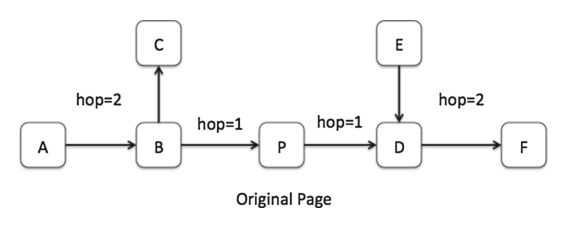
\includegraphics[scale=0.95]{Figures/GenreSim_Draw.eps}
		\caption{GenreSim page selection diagram, found in  \parencite{zhu2016exploiting}.}
		\label{fiig:GenreSim_Draw}
	\end{center}
\end{figure}

GenreSim is a ranking algorithm based on PageSim algorithm, extended to fit in the problem of genre-taxonomy. Similarly to all this kind of algorithms, is based on the assumption where the more webpages refereed to a particular webpage the more this page is related to them in class of topic and/or genre taxonomy. Respectively to the genre-taxonomy the assumption for the GenreSim algorithm this relation is expended to the level of \textit{forward} $F(p)$ and \textit{backwards} $B(p)$ related URL links. Moreover, the web-pages URL structure is also scored and the pages are characterized as \textit{Hubs} $H(p)$ ans \textit{Authorities} $A(p)$. The null hypothesis of the algorithm is than web pages of the same genre are inter-connected with their URL links, thus as small network of a few pages backwards and forwards to a specific web-page consists a "small" network of the same genre. Thus, using the textual and partially the structural information of these selected neighbour pages will amplify the information required to classify this page to the proper genre.

Particularly Hubs are pages with many outgoing URLs, whereas pages with many URLs pointing to the are called authorities. The number of incoming and outgoing URLs are increasing the respective scores as shown in equation \ref{eq:GenreSim_hub_authortities}. However, web-pages with high score but with \textit{few backward URL links} its high likely to be "spam" pages in the context of genre relation. In order to regulate this the $\omega(p)$ factor is intruded of equation \ref{eq:GenreSim_omega}, where is reducing the score for the web pages with few backward links, where is also normalizing the "few links" issue. That is the number of the backward links is correlated to the number of links the page it self is containing. 

\begin{equation}\label{eq:GenreSim_hub_authortities}
	\begin{array}{l}
		H(p) = \sum_{u \in V|p \to u} \omega(p) A(u) \\  
    	A(p) = \sum_{v \in V|v \to v} \omega(p) H(u) \\
    \end{array}
\end{equation}
\begin{equation}\label{eq:GenreSim_omega}
	\omega(p) = \frac{N}{|\log N - \log N(p) | + 1} 
\end{equation}
Therefore for a random webpage in the $G$ graph of web-pages, its score is calculated by equation \ref{eq:GenreSim_Score}. In general the \textit{genre-selection recommendation score} is propagated to the graph path $P(u,v)$ as indicated by the $Score(u, v)$ function of equation \ref{eq:GenreSim_Path}. Thus the recommended webpage's score to be selected is decreasing gradually as the recommended pages is farther (in hops) from the web-page to be classified. The $d$ factor is set to be $0.5$, i.e. the page score is decreasing by half for every hop farther from the page under evaluation. 

\begin{equation}\label{eq:GenreSim_Score}
	Score(p) = H(p) + A(p)
\end{equation}

\begin{equation}\label{eq:GenreSim_Path}
	Score(u, v) =
      \begin{cases}
      	\sum_{p \in P(u, v)} \frac{d Score(u)}{\prod_{x \in p, x  \neq v} (|F(x)| +|B(x)|)}, & v \neq u \\
        Score(u), & v = u \\ 
       \end{cases}
\end{equation}
Finally, the similarity of the candidate neighbour pages to the one under evaluation is calculated form equation \ref{eq:GenreSim_Selection_Score}, which is the ration of the min and the max paths-score sums of all the possible paths, backwards and forwards, to the page under evaluation.

\begin{equation}\label{eq:GenreSim_Selection_Score}
	Sim(u, v) = \frac{\sum_{i=1}^{n} min(Score(v_{i}, u), Score(v_{i}, v))}{\sum_{i=1}^{n} man(Score(v_{i}, u), Score(v_{i}, v))}
\end{equation}
GenreSim is combined with an ML algorithm called MCC (Multiple Classifier Combination). Particularly GenreSim utility is to select a set of webpages where their content (textual and structural) will be used in combination to the "on-page" content as an input to the MCC algorithm for classification of a random webpage to a Genre-taxonomy.

The MCC algorithm is a set of SVM classifiers where each is trained to a particular set of features from the webpage and its neighbours, well selected from the GenreSim, webpages. Then a Decision Template, shown in equation \ref{}, is build and used for the classification of random webpage. Then the Min, Max or Mid values for the classification decision from the matrix are selected for making the final decision for the Genre class of the web-page.

\begin{equation}\label{eq:GenreSim_DP}
	DP(p) = \left(
    	\begin{array}{ccc}
        	d_{11} (p) & \cdots & d_{1|G|} (p) \\
            d_{21} (p) & \cdots  & d_{2|G|} (p) \\
            & \vdots & \\
            d_{N1} (p) & \cdots  & d_{N|G|} (p) \\
         \end{array}
\right)
\end{equation}
Where $|G|$ is the number of genres in a genre taxonomy and the calcification methods is under a closed set setup with $N$ indented (one for each feature set) \textit{SVM multi-class classifier}. 

\section{Focused Crawlers for Genres}\label{chap:relevant_work:sec:intro}

\section{Genres Utility}\label{chap:relevant_work:sec:intro}
journalism historians
Genres variations on students writing...

An other study related to the utility of the genre taxonomy of the \textit{Search Engines Results (SER} is one conducted at Pittsburgh, USA, University.  The experiment measured the correlation of the website's/web-page's genre and the user's preference for completing the task of finding health care information for Multiple Sclerosis and Weight Loss. The results clearly show that the user's task would be significantly easier if the web resource were organized based on their genre and no only on their topic relation ranking \parencite{chi2018sources}.

An other TEXT-GENRE identification utility is for video (e.g. movies, TV series, etc) classification in video/cinematographic genres using the text available such as the subtitles. In this study a variety of ML algorithms has been tested such as SVM, Naive Bayes, Random Forest, Decision Trees and several types of features. Features usually called superficial here where called \textit{content-free} and the ones related to specific words called \textit{content-specific}\parencite{lee2017text}.

As reported in \parencite{rangel2016overview} which is a work related to \textit{Author Profiling}, a cross-genre evaluation has been employed. That is, texts from a variate of different genres such as \textit{Social Media, Blogs, Twitter and Hotel reviews} used for this task's evaluation. Therefore, an automated WGI methods would be really useful for collected fast training data or experimental data sets for such tasks.

An other utility is the AGI/WGI for \textit{office/local documents}, i.e. pdf, images (jpg, png, etc), slides (Powerpoint, Keynote), HTML based tutorials/booklets etc. There is at least one experimental application where in a multi-faceted search/browsing application for locating local documents in an office environment (with shared files) was using an open-set  genre-taxonomy for aiding the users locating their files. Particularly, their application was accepted form the users who tested it and they reported than using the genre-taxonomy filtering they have managed to locate old slides abandoned more than a decayed related to their current work. As explained above they where using an ensemble based algorithm within an open-set framework which was trained in a relatively small data-set of 5,098 pages, while it was tested in a production environment with 30,000 office documents of a 10-year time span \parencite{chen2012genre}. 

\section{Web Genre Temporal Property}\label{chap:relevant_work:sec:intro}

The temporal idiosyncrasy is also an major  

Moreover the  and the context of the text and \textit{the groups defining, forming, and using the genre tag/category}.

Related to the web genre-types, in the very early studies it has been pointed out that the users are the most important component of the research. 

An other study advocating in the temporal manner of the web-genre is the one of  \parencite{caple2017genre} where they show how News web-genre changed overtime and additionally new sub-genres potentially occurred.

Jebary SOS



\section{Deep Learning Vocabulary of Distributional Features for WGI and WGC}\label{chap:relevant_work:sec:intro}


PRIMITIVE DISTRIBUTIONAL \parencite{kim2010formulating} 


The state-of-the-art in the text-genre classification and WGI/WGC is the Vocabulary-Learning ans particularly the use of the deep-learning methods for building comprehensive-abstract-term vocabularies. This methods due to the nature of the Neural-Networks, mainly used,  the procedure for building vocabulary-models is implicitly embedding a variate of information syntactical, morphological or even structural. However there are some efforts where an explicit use of this kind of information use exploited for the classification task. 

A combination of BOW, superficial and syntactical features. \textit{Content-free} (a.ka. superficial) features in combination with specific words called \textit{content-specific} has been test for genre classification. These feature have been used as an input to a variety of learners such as SVM, Random Forests, Decision trees, Naive Bayes etc with significantly high performance. However, they found that the combination of the features was more efficient when it was combined using a meta-classifier than using a \textit{supervector} containing a sequence of all the features together. Particularly, the where training a different learning for a different set of features and then they were fiddling the results to meta-learner\parencite{lee2017text}.

Their method resembles the deep-learning method of building a DF vocabulary model where afterwords its output is fed to an other classifier. However, this methods can be characterized as Explicate Vocabulary Modeling (EVM) compare to the implicate vocabulary modeling (IVM) when deep learning methods are used.

There are some pros and cons comparing EVM methods to IVM. The main advantage of the "explicit" methods is that they enabling us to figure out which part of the information was really important thus to reduce the computational effort by removing the prepossess of information that is redundant or even causing confusing. On the other hand we have explicitly have to figure out which information to capture, while in the IVM there is no such a need. (THINK THIS STATEMENT AGAIN)

In their study compared their method to in both cases of \textit{binary} and \textit{tf (term frequency)} (Kanaris-Stamatatos)
....
....
....
The state-of-the art relate to the Word-Vectors Learning Models, i.e. the \textit{Deep Learning (Neural Based Models)} or \textit{Pointwize Mutual Information (PMI)}, is the Post-processing of the resulting modeled vectors. Such example is the \textit{unsupervised Post-processing via Conceptors (or Conceptor Negation)}. The main concept is to suppress the outages frequencies using PCA, SVD and most recently Conceptors Negation. The latest is a methodology (unsupervised) of Conceptors are a family of regularized identity maps introduced by (Jaeger 2014 ???) where a linear transformation is taking place minimizing a loss function similar to the PCA process. However, this methodology on the contrary to the PCA is a "Soft" regularization or "Soft" noise filtering, while PCA is considered "Hard". In both cases by projecting the data-point to the prediction space we are able to filter the noise or outages samples. Intuitively, these methods are post-processing the distributional feature vectors in order to enrich their semantic content. Moreover, using the "soft" noise reduction filtering (CITE Unsupervised Post-processing of Word Vectors via Conceptor Negation ).

Then \textit{n-gram term types} for WPGC problem proposed by a series of papers by Manson et al.\parencite{mason2009n,mason2009classifying,mason2009distance}. In their studies were comparing their method to previous studies on WPGC based on n-grams and they have tested their approach on the range of 2-grams to 10-grams. The learning models under comparison was SVM, k-Nearest Neighbors, and a distance based method they proposed. Their approach uses a distance measure from the domain of \textit{Author Identification} and they used this measure with three different representation of the genre classes. In oder to form the a prediction class, using this their method, were getting the vectors of the training sample and forming a centroid(characteristic) vector. Then an arbitrary web page vector were compared to the characteristic vector with the distance measure in order to be classified. Their approach was comparable to other methods, however, SVM had shown better performance. In their work studied two methods of selecting the genre features for discriminating the pages, one by keeping an $z$ number of the most frequent features within the genre training corpus. The second feature approach was the use of the \textit{chi-square statistic} ($\chi^{2}$), which performed \textit{statistical significantly} better than \textit{frequency based selection}. It is important to note that their series of works was extensively examined the influence of n-grams size to the performance of the prediction models and they have shown that there is a statistical
significantly difference between the different sizes.

There is an other study from Dong et al.\parencite{dong2006binary} focusing on the measures that could potentially used for feature selection in the context of WPGC. The have tested\textit{ chi-square statistic} ($\chi^{2}$), Information Gain and Mutual Information over three samples sets of three different genres. Each of the evaluation data sets for every genre, was composed from pages related to the genre and random pages. Their experiments were binary classification tasks using Naive Bayes, SVM, and Neural network classifiers. Irrespectivelly of the classifiers all the statistical measures used for feature selection had similarly good performance. The feature size they used was 5, 20 and 100 features, where for 20 and 100 the results had no statistically significant difference. The term vectors or the web pages where binary formatted.


""Examples of word vectors include Word2Vec (Mikolov et al. 2013), GloVe (Pennington, Socher, and Manning 2014), Eigenwords (Dhillon, Foster,and Ungar 2015), and Fasttext (Bojanowski et al. 2017). These word vectors are usually referred to as distributional word vectors, as their training methods rely on the distributional hypothesis of semantics (Firth 1957)."""


\section{Using the Web as a Corpus - The Genre Approach}\label{chap:relevant_work:sec:intro}

\section{Genre Research outside pure CS (???)}\label{chap:relevant_work:sec:intro}


\section{The Web Genre units: Section, Page, Site}

In all studies it was pointed out that in most cases in a webpages or in a text usually there are multiple genres.... \parencite{lee2017text} (also Ashegi, Santini, and other old citations).


\section{Web Genre Corpora: An unfinished work in progress}\label{chap:relevant_work:sec:intro}

The constitution process for the rules required to be followed for composing a text corpus is still a research problem in \textit{linguistics studies}, while the utility of the genre-taxonomy is vividly pointed out. A collection of texts cannot be assumed to be a corpus by default due to several issues should be considered starting with the taxonomy definition where mostly is an overlapping problem, then the texts should have several properties linguistically and statistically defined. The homogeneity in temporal manner, whether are from multiple languages and the way have been collected; \textit{speech, spoken or written corpus}. Particularly speech corpus implies voice recording while spoken means to be transcribed from speech samples. Particularly for the genre-taxonomy the homogeneity related to the time samples has been collected is very critical since the genres are changing over time until a new genre occurs replacing or dividing from an older \parencite{dash2018history}. Blogs, for example, was the evolution of "personal/memory diaries" when they became public on the web and named "web-logs" then in a second time evolution renamed to "blogs" where their content also changed now is mostly like an \textit{informal journalism} rather than a diary.

The NLP community has overcome, by ignoring mostly, the problem of a non-well established corpus of the WGI, and in general for the \textit{Text Genre Identification}. There are at least tree publication on the effort on \textit{corpus building methodologies} with vividly different approaches, yet the problem is remaining open due to several issues described in detail in section
\ref{chap:relevant_work:sec:linguistics_definition} and in \parencite{melissourgou2017genre,asheghi2014semi (Ashegi,2018_Book_HistoryFeaturesAndTypologyOfLa_WEB_TEXT_CORPUS.pdf). 

All the approaches are focusing on the genre's main principals, i.e. the function, form and communicative purpose. While in \cite{asheghi2014semi} the focus was on the semi-automated evaluation procedure in the categorization of the texts, in \parencite{melissourgou2017genre} the process is focusing on the systematic manual process.  This process is based on a well established theory of  the Systemic Functional Linguistic (STL) framework where as a shortcut in the process can help on building and evaluating a genre taxonomy corpus. 

There is no drought for the significant contribution of the above studies where all three can be used as the solid framework for building \textit{web-genre-taxonomy corpora} and web-text corpora in general. The utility of the each work can be used as multi-layer filtering process:  1) starting with the automated crawling of the web using focused crawling as explained above \ref{}, 2) Using non-experts crowd-sourcing semi-automated procedures form first level filtering, 3) using the methodology of manual STL based evaluation for fast qualitative analysis and categorization of the post-crowdsourcing-filtered corpus. 

Starting form the final step \parencite{melissourgou2017genre} work firstly is resolving the ambiguity on the notions related to genre. As they explained the terms "genre", "register", and "text type" are used interchangeably, complimentary and even contradictory, plus to the debate related to the terms usage. However, in general there terms it turns out to be subsets and super-sets of one to the other. Particularly \textit{text's register, communicative purpose, form} are all components of the \textit{text's genre}, while \textit{text type} is mainly defined by the \textit{text's form}. Alternatively, register is used to describe very general concepts of writing styles such as \textit{formal/informal} while genre mostly includes also the purpose such as \textit{news/blog}, where news' style is mostly formal and blog's infomal. Moreover, text's form is also one of the three components of the \textit{register} where then is called "mode". One could attempt to describe the connection of these terms in a mathematical equations such as in eq.  

\begin{equation}\label{eq:genre_notion_in_math}
	G  \subseteq P \uplus F \uplus T \uplus M
\end{equation}
where $G$ is the genre, $P$ is the communicative purpose and $F, T, M$ are the "register's" components. $F$ is the \textit{field} which answers to the question of \textit{Why?} the text was composed. $T$ is the \textit{tenor} which answers the question of \textit{Who?} or/and to \textit{Whom?} the text was written. $M$ is the \textit{mode} which is the text's form. Note, that G is not exactly equal to their sum of these components of the text, because, as it has also mentioned before in this thesis although the text's context we would like to be orthogonal to the genre - since is mostly related to the topic - yet there are some contextual text peaces that are critical for the genre identification, exactly as it was happening in the cognitive experiments on genre identification of \parencite{clark2014you, lieungnapar2017genre} (briefly explained in section \ref{chap:relevant_work:sec:linguistics_definition}).

An other interesting path towards to the process automating the building of Genre-Taxonomy corpora is the one found in \parencite{lieungnapar2017genre}. They are using a simple K-means clustering method for finding an automated procedure for capturing the possible correlation of \textit{logistic features} and the \textit{Popular Science Sub-Genres}. In their methodology they are using set of manually extracted linguistic features as presented in table \ref{chap:relevant_work:tbl:pop_science_features} and then they are correlating the z-scores of these features to the possible 4 clusters found to be in the Popular Science \textit{web documents}. Following the same strategy they have managed to show the correlation of the sub-genres to the science disciplines and document sources. Finally they have managed to correlate manually identified genre's function to the linguistic features. Showing that it is possible by using a short of \textit{Funnel like Filter} is possible to gradually extract higher and more abstract levels of information starting with the linguistic features, conginuing with function features (or text-registers) (e.g. Impersonal, Narrative, Persuasive, Informative, Elaborated, Impersonal) and finally classifying the genres. Finally, they have shown that their final evaluation to their, obviously, semi-automated process was as good as the experts agreement on the same task after they have manged to form a "golden standard" manually. 




\section{Discussion}

AGI/AGC and particularly WGI is a complex problem for NLP ( and in computational linguistics in general) where several approaches has been proposed in the effort to tackle this task. All the above faceted survey giving us a fruitfully information set where we should put it into an order and derive a conclusion where it could help the AGI research to go several steps forward. Particularly here it is assumed that eventually the linguistic research will converge to the NLP in the direction of creating rich genre-taxonomy corpora by using semi-automated methods and most importantly a well defined methodology to assess and constitute them properly. Thus by overcoming this bottle neck here it is discussed the potential directions for the AGI task.

Feature selection and document representation independently or combined with the classification/identification ML method seem to be the main problem most of the researchers are primarily trying to tackle. In section \ref{chap:relevant_work:sec:features} there is a great amount of work on heuristic methods for capturing the amount of information for enabling any out-of-the box ML method (or special version of it) to identify the genres of a genre-taxonomy. The whole effort of more than a decade on the feature selection leading as in two main conclusions. The \textit{power of words} and the \textit{language dependency}.

The power of words, in the sense that in all the cases of (see tables .....) it seems than there are words with a great "informative energy" and they can even define the genre when they are present on the URL of the web page (see work of identify web-genre using URL). In addition there are cases where this words although they are tightly connected to the context they are indicators also for genre-identification (see study for POP-Science sub-genres). Finally, using DF features it seems again that words are good enough for returning all the information required for the AGI task. 

On the other hand sine the words are so powerful they are tightly connected to the language where the text is written. Thus all these ML automated proposals are potentially canceled when the language is written. Moreover, superficial text information, such as colon frequency, document length, sentence mean length, and single-sentence paragraph count, seems to work fine in cases of cross-lingual genre classification such as in the case of \parencite{nguyen2019cross}. 

To this end in feature selection and document representation the research seem to be  required to focusing in generalized representations not necessarily superficial based but mostly in feature selection methods where they can be used in any language and ideally cross-lingual. Again DF features seems one of the research paths one could be follow for the AGI.

Based on the DF features paradigm \textit{sampling in several text properties} in character, word, paragraph, text level seems to be a path to follow especially in a case where an ML algorithm could do that as a part of the its whole optimization procedure, from the raw text.

The ML methods experimental framework in respect of closed-set and open-set is an other very import aspect for the AGI....

























